\chapter{\label{chp:background}Theory and previous work}
Theory, background and previous work is important to give a thurow understanding of the material to follow in the next chapters. The base of this background chapter is written as part of the specialization project conducted during the autumn of 2015, but it is included here to allow the report to be a freestanding document and to add a deeper level of explanation of some of the described concepts than that presented in the previous report. 
In the early days of digital hardware design, gate design and layout were performed by hand. With the rapid growth in the numbers of transistors per digital chip-design, this method quickly became too time-consuming and the need for new and more automated design methods rose. \gls{rtl}-design using \gls{hdl} has long been the standard in digital hardware design. With the increasing demand for low power and small area in large \gls{soc} designs with multiple billion transistors, this methodology is no longer sufficient if hardware manufacturers want to hit the window of opportunity with their state-of-the-art product.

\section{\label{sec:hls}High-Level Synthesis}

\gls{hls} is not a new concept as it were introduced in research papers in the late 1970s and further researched and developed in the 1980s and early 1990s \cite{martin2009high}. The available commercial \gls{hls} tools have not been providing the necessary performance and benefits over \gls{hdl} development for major hardware development companies to adapt this methodology until recently.
The concept of \gls{hls} starts with a functional specification of the circuit described using a higher abstraction level, often a \gls{hll}. A tool use target architectural model libraries and design constraints to transform this specification into hardware, represented as a \gls{rtl} or \gls{hdl}-model. The typical \gls{hls}-flow is shown in figure \ref{fig:hlsflow} and each of the transition-steps is described in the below subsections. The input libraries contain information on available hardware resources with power, area, and delay models for the target architecture.

\begin{figure}[hbpt]
\centering
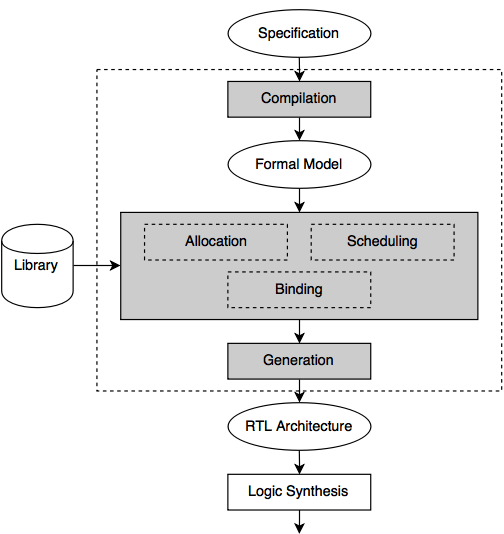
\includegraphics[width=0.55\textwidth]{../figs/HLSFlow.png}
\caption{\label{fig:hlsflow}Information flow in a typical HLS-tool \cite{coussy2009introduction}.}
\end{figure}

\subsubsection{Compilation}

The first step of \gls{hls} is to compile the functional specification into a formal model. This model can vary between different tools, and can be either a specific representation language or a graphic representation of the flow. The formal model is decided by the developers of the \gls{hls} tool. 

\subsubsection{Allocation}

Necessary hardware resources, such as functional units, storage-, and connectivity-components needs to be selected from a given \gls{rtl} component library in order to satisfy the specification and design constraints. Some \gls{hls} tools can also add more resources in the scheduling and binding tasks, if this is needed to meet given constraints.

\subsubsection{Scheduling}
Scheduling arranges all operations in an optimized sequence so that variables are read from sources and brought to the input of the correct functional unit for execution and to the destination afterwards. The scheduler takes all dependencies into account when scheduling the operations, in order to get the most efficient result, as some operations can be executed in parallel if no dependencies exist and there is available resources. Operations can be scheduled to finish in one, or take multiple clock-cycles, and operations can also be chained to eliminate the need for storing the result between operations, and to reduce the total number of cycles needed. 
\subsubsection{Binding}
In the binding task, all clock-cycle-crossing variables, operations, and transfers are bound to a free resource, in the time-frame when it is scheduled. Non-overlapping or mutually exclusive variables can be bound to the the same storage unit, and operations can be bound to the best optimized functional unit if multiple alternatives are available. Each transfer from component to component, either storage or functional unit, needs to be bound to a connection unit, such as a bus or a multiplexer.
\subsubsection{RTL Generation}
The generated \gls{rtl} usually consists of two parts, a control-unit and a data-path-unit. The control-unit is often implemented as a \gls{fsm}, which set control-signals to the data-path, and controls the current and next-state of the system. The data-path contains storage-, functional-, and connection-units. Depending on the intensiveness of the binding step, the output \gls{rtl} can be tightly or loosely bound to the available resources. If an operation is not bound to a specific unit, it is up to the following logic synthesis of the \gls{rtl} to bind the operations to available resources. The different types of \gls{rtl} output are illustrated by the following example. \textit{a = b * c} executing in state \textit{n}:

\begin{minipage}[t][300px]{\textwidth}
\textbf{Without any binding:}%\hfill\vspace{-\baselineskip}
\begin{verbatim}
state (n): a = b * c;
go to state (n + 1);
\end{verbatim}
\textbf{With storage binding:}%\hfill\vspace{-\baselineskip}
\begin{verbatim}
state (n): S(1) = S(2) * S(3);
go to state (n + 1);
\end{verbatim}
\textbf{With functional-unit binding:}%\hfill\vspace{-\baselineskip}
\begin{verbatim}
state (n): a = MUL1 (b, c);
go to state (n + 1);
\end{verbatim}
\textbf{With storage and functional-unit binding:}%\hfill\vspace{-\baselineskip}
\begin{verbatim}
state (n): S(1)=MUL1 (S(2), S(3));
go to state (n + 1);
\end{verbatim}
\textbf{With storage, functional-unit, and connectivity binding:}%\hfill\vspace{-\baselineskip}
\begin{verbatim}
state (n): BUS1 = S(2); BUS2 = S(3);
BUS3 = MUL1 (BUS1, BUS2);
S(1) = BUS3;
go to state (n + 1);
\end{verbatim}
\end{minipage}

A loosely bound \gls{rtl} gives the synthesis-tool the flexibility to optimize the unit binding to updated timing estimates, delays, and loads given by the layout and floor-planning tools.

\section{LegUp}
The \gls{hls} tool used in this project is called LegUp \cite{canis2011legup}. LegUp is an open-source academic tool developed at the University of Toronto, Canada. LegUp's goal is to \textit{"allow researchers to experiment with new \gls{hls} algorithms without building a new infrastructure from scratch"} and their long-term vision is to \textit{"make \gls{fpga} programming easier for software developers"}. LegUp takes \gls{ansi}-C as input and generates synthesizable Verilog \gls{hdl} as output. The developers of LegUp have primarily focused on support for a variety of \gls{fpga} boards from manufacturer Altera, but in the latest version (4.0), beta support for Xilinx devices and possibility to configure the tool to generate generic Verilog to target other \gls{fpga} vendors or even \gls{asic} through use of generic dividers, has been introduced. The big advantage of LegUp compared to similar, commercial tools, is that it is open-source and therefore can be configured to target different architectures. The \gls{rtl} and \gls{hdl} generating part of the tool can be modified or replaced to fit the programmers needs.
Since LegUp, in its unmodified form, target \gls{fpga} devices, it support three different synthesis flows; pure-\gls{sw}, hybrid, and pure-\gls{hw}. The two first synthesis flows will implement a TigerMIPS \cite{tigmips} soft processor, which will run part of the C code. The partitioning of \gls{sw} and \gls{hw} in the individual modules are described in \cref{tab:legupflows}. It is the pure-\gls{hw} flow that will be the focus of this project.

\begin{table}[hbpt]
    \centering
    \caption{\label{tab:legupflows}HLS-flows supported by LegUp and partitioning between SW and HW}
    \begin{tabular}{lp{4.8cm}p{4.8cm}}
      \textbf{Flow} & \textbf{Functions run in hardware} & \textbf{Functions run in software}\\
      \toprule
      Pure-SW & None & All \\
      \hline
      Hybrid & Specified hardware-accelerated functions & All other functions \\
      \hline
      Pure-HW & All & None\\
      \bottomrule
    \end{tabular}
\end{table}

\subsubsection{Producing Verilog Output}
LegUp is made up of two components; a frontend pass and a target backend pass to the LLVM compiler infrastructure. 
The information flow in LegUp, shown in figure \ref{fig:legupflow}, follows the same principle as the information flow described in section \ref{sec:hls}.
\begin{figure}[hbpt]
\centering
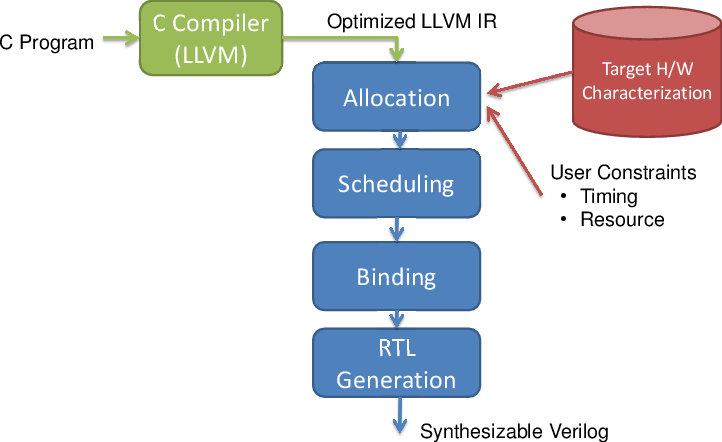
\includegraphics[width=0.6\textwidth]{../figs/LegUpFlow.png}
\caption{\label{fig:legupflow}Information flow in LegUp \cite{legupmaual}.}
\end{figure}
The LegUp LLVM frontend takes LLVM-\gls{ir} compiled by clang, a C frontend for LLVM, as input and links in custom written functions like memcpy, memset and memmove, which do not exist in hardware, but that LLVM assumes exist in the C library. 
The LegUp backend pass performs allocation, scheduling and binding as described in section \ref{sec:hls}. In the next step, \gls{rtl}-module objects that represents the final hardware circuit are generated from each LLVM instruction. Ultimately, Verilog code corresponding to each of the \gls{rtl}-modules is output to a file.

\section{\label{sec:LLVM}LLVM}
LLVM \cite{LLVM:CGO04}, formerly Low-Level Virtual Machine, is a compiler framework that was originally developed as a research infrastructure to investigate dynamic compilation techniques for static and dynamic programming languages, at the University of Illinois in 2000. It is now a open-source project with many contributors from both industry, research groups and individuals, and it is used by companies like Apple in their Xcode \gls{ide} \cite{llvmapple} and Sony for their PS4 developer toolchain \cite{llvmsony}. LLVM support a large number of frontends for programming languages, including Clang \cite{clang} which support C, C++, Obcjective-C, and Objective-C++, and is compatible with \gls{gcc}. It also supports a large number of backend target architectures. Figure \ref{fig:llvmcompiler} shows how different source languages can be input to the frontend compilers of LLVM, which translate the source into an \gls{ir}. The \gls{ir} is then optimized using LLVM's optimizer. At this stage, different source languages can be linked together, and even object files compiled using standard \gls{gcc} can be linked at this stage. The optimized \gls{ir} is then translated into the target architecture by the backend.

\begin{figure}[hbpt]
\centering
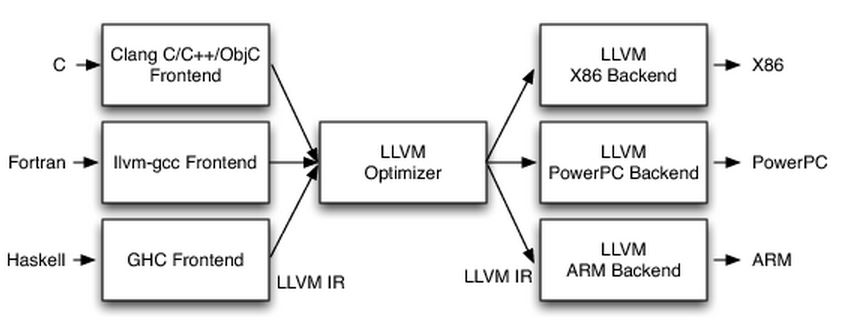
\includegraphics[width=\textwidth]{../figs/LLVMCompiler.jpg}
\caption{\label{fig:llvmcompiler}LLVM's three-phase compiler structure \cite{llvmarch}.}
\end{figure}

\subsubsection{Intermediate Representation}
LLVM use a human readable assembly-like, strongly typed RISC instruction set as their \gls{ir}, with support for an infinite number of temporary registers of the form \%0, \%1, etc. LLVM-\gls{ir} can also output a dense bitcode format for serialization.

\section{Alternative hardware design methods}
\gls{hls} is not the only alternative to \gls{hdl}-languages, if you want to design digital hardware at a higher level of abstraction. The following subsections will shortly describe two alternative approaches to digital hardware design. 
\subsection{Chisel}
One interesting approach to designing hardware with a higher level of abstraction, is the Chisel \gls{hcl} \cite{bachrach2012chisel}, developed at UC Berkeley. Unlike \gls{hdl} languages like VHDL and Verilog, which were originally designed as simulation languages and later adopted as a basic for synthesis, Chisel was created as a \gls{hcl} and is thus \textit{synthesizable by construction}. This entails that no conversion from C, or other \gls{hll}, into gates is performed, only generation of generic low-level Verilog with no overhead. Chisel is a \gls{dsl} built on Scala \cite{odersky2004overview} with its own syntax, but Scala syntax can also be used to get even greater abstraction in your design. A big advantage using Chisel is its high simulation speed, using C++-based cycle-accurate software simulators.

\subsection{Functional programming}
Functional programming is a relatively different method of hardware design, as it consists only of mathematical functions and immutable data. Two examples of hardware design using functional programming is C$\lambda$aSH \cite{baaij2009clash} and Lava \cite{bjesse1998lava}. Both Lava and C$\lambda$ash are compilers for the functional programming language Haskell \cite{haskellonline}, but while Lava is an embedded \gls{dsl} like Chisel, with its own syntax, C$\lambda$ash use Haskell syntax and semantics, and use a static analysis approach towards synthesis.

\section{Programming concepts}
In high-level programming languages like C and C++ and in \gls{hdl} languages like Verilog, the use of programming concepts are extensively used. This section describes some concepts that are frequently referred throughout this report.
\subsection{Structures}
A structure, or struct for short, is a complex data-type that can contain multiple other variables of different data-types. 
\subsection{Classes}

\subsection{Pointers}
A pointer is a variable that is defined to point at a location in memory where another object is stores. The pointer itself contains the memory address of the object it points at.
\subsection{Declaration}
Declaration refers to the process of declaring a type or an object that will be used at a later stage. This can be a structure in C, a Class in C++ or a module in Verilog. A type or an object needs only to be declared once and can then be used as many times as necessary. An example of a declaration of a struct in C: 
\lstset{language=C++, style=Cstyle}
\begin{lstlisting}
typedef struct Book_t { char title[128], 
                        char author[128], 
                        int isbn 
                      } Book;
\end{lstlisting}
By declaring the struct using \textit{typedef}, the struct can be instantiated by writing only the type-name and the variable name \verb!Book myBook!, instead of writing \verb!struct Book_t myBook!.
\subsection{Instantiation}
Instantiation is when the object you created with your declaration, is created and stored at a designated location in memory. When you instantiate an object, you usually assigns it a variable, or name, that you use throughout the scope of the object to reference the object.
\subsection{Assignment}
Assignment means to assign a value to the instantiated object.

\section{\label{sec:legupclasses}LegUp classes}
LegUp has some predefined classes that is important for the understanding of the following description of how the issues in LegUp are resolved. The following subsections will describe these classes in more detail.
\subsection{RTLModule}
The RTLModule class models a hardware RTL module. The class stores information about all ports (inputs and outputs), signals, parameters and sub-modules. Each function declared in the C-code transforms into a RTLModule object. Each function that is called from the function will be added as a sub-module to the RTLModule object, meaning a module instantiation will be added to the module. Important member functions in the RTLModule class is:
\begin{compactdesc}
    \item[getName()] \hfill \\
    Returns a string containing the name of the RTLModule, i.e. "main" for the module generated by the main-function in the C-program.
    \item[find(std::string signal)] \hfill \\
    Takes a string containing a signal name as parameter and returns a pointer to the RTLSignal in the RTLModule with that name.
    \item[addParam()] \hfill \\
    Adds a parameter to the module. The function returns a pointer to the generated RTLSignal object.
    \item[addIn()] \hfill \\
    Adds an input port to the module. The function returns a pointer to the generated RTLSignal object.
    \item[addOut()] \hfill \\
    Adds an output port to the module. The function returns a pointer to the generated RTLSignal object.
    \item[addRegOut()] \hfill \\
    Adds a registered output port to the module. The function returns a pointer to the generated RTLSignal object.
    \item[addReg()] \hfill \\
    Adds a register signal to the module. The function returns a pointer to the generated RTLSignal object.
    \item[addWire()] \hfill \\
    Adds a wire signal to the module. The function returns a pointer to the generated RTLSignal object.
    \item[addModule()] \hfill \\
    Adds a instantiation of another module to the module. The function returns a pointer to the generated RTLModule
    object.
\end{compactdesc}
\subsection{RTLSignal}
The RTLSignal class represents the signals within an RTLModule. Both internal signals, port signals and condition signals are all modelled usign the RTLSignal class. Important member functions of the class is:
\begin{compactdesc}
    \item[getName()] \hfill \\
    Returns a string containing the name of the RTLSignal, i.e. "clk" for the clock signal.
    \item[getType()] \hfill \\
    Returns a string describing the signal type. The type can be reg, wire, input, output and output reg.
    \item[getNumDrivers()] \hfill \\
    Return the number of driving RTLSignals. 
    \item[getDriver(unsigned i)] \hfill \\
    Returns a pointer to the i-th driving RTLSignal.
    \item[getCondition(unsigned i)] \hfill \\
    Returns a pointer to the condition signal of the i-th driving RTLSignal.
    \item[addCondition(RTLSignal *cond, RTLSignal *driver)] \hfill \\
    Adds a conditional driver. If the RTLSignal \textit{cond} is true, the RTLSignal \textit{driver} drives the signal. 
    \item[connect(RTLSignal *s)] \hfill \\
    Connect this signal unconditionally to another RTLSignal.
    \item[getWidth()] \hfill \\
    Returns a pointer to a RTLWidth object, describing the width of the RTLSignal.
    \item[isOp()] \hfill \\
    Returns true if the RTLSignal is an RTLOp object.
\end{compactdesc}
\subsection{RTLOp}
The RTLOp class is a subclass of the RTLSignal class, representing an operation with one, two or three operands. Each operand is a RTLSignal. The operation can be an arithmetic operation like addition, subtraction, multiplication, or division, and it can also be logical operations like AND, OR, and XOR, or even comparison operations like equal, not equal, less than, less than or equal, greater than, and greater than or equal. The whole list can be seen in the class reference \cite{rtlopclassref}. A RTLOp object modelleing an AND operation of two operands, operand1 and operand2, will in Verilog correspond to the operation \verb!operand1 & operand2!. Some important member functions are:
\begin{compactdesc}
    \item[getOperand(int i)] \hfill \\
    Returns a pointer to i-th operand of the RTLOp object.
    \item[getNumOperands()] \hfill \\
    Returns the number of operands of the RTLOp object.
    \item[setOperand(int i, RTLSignal *s)] \hfill \\
    Sets the i-th operand to the RTLSignal \textit{s}.
\end{compactdesc}
\subsection{RTLWidth}
The RTLWidth class represents the bitwidth of a RTLSignal. An RTLWidth is defined by high and low bits, for instance 31,0 for a 32 bit signal. This will transform into \verb![31:0]! in Verilog.
\subsection{RAM}
The RAM class models RAM modules in LegUp. Whenever a variable is loaded or stored, a RAM module is generated to handle the loads and stores. The RAM objects can be divided into two scopes; LOCAL and GLOBAL. A Local RAM object is local to a given function and cannot be accessed from other functions. A global RAM object will be implemented in a global memory controller, and all modules that use the variable can connect to the RAM via the memory controller. Some important member functions are:
\begin{compactdesc}
    \item[getName()] \hfill \\
    Returns a string containing the name of the RTLModule, i.e. "main\_0\_1" for the RAM module generated for the first parameter to the main function declared as volatile (output parameters) in the C-code.
    \item[isROM()] \hfill \\
    Returns true if the RAM is read-only.
    \item[getScope()] \hfill \\
    Returns if the RAM is in the local or global scope.
\end{compactdesc}

\section{\label{sec:powest}Power and area estimation}
In order to compare different use-cases and result generated by LegUp, the area usage and power consumption will be estimated. Since this is not the main objective of this project, the automated area and power estimation tool-flow created by Joar Talstad in his specialization project \cite{talstad14project} and master thesis \cite{talstad15master} will be adapted for this purpose. This tool-flow use Synopsys Primetime PX for power analysis and estimation.

\section{Information- and tool-flow}
LegUp utilizes Makefiles to perform the \gls{hls}-flow. The power and area estimation tool-flow described in section \ref{sec:powest} also use Makefiles for its flow. It can therefore be clever to create a single Makefile that controls the information-flow from the input of C-files to the output of Verilog-files along with score-files of area and power estimates. 

\section{Reference designs}
\label{sec:refdes}
In order to evaluate the performance and overhead in power and area generated by LegUp, two reference designs are created to compare the produced results from LegUp towards the same design written in native Verilog \gls{hdl}. To evaluate whether the structure of the design impact the overhead on the output, the first design contains a regular structure, where the same operations are performed each clock-cycle. The first reference design was chosen to be a \gls{fir}-filter. The second design contains a state machine, as it is interesting to see if the \gls{fsm} implemented by LegUp generates less overhead if the design itself is a state machine. The choice landed on designing a \gls{sap-1} architecture. Both designs are described in the subsections below.

\subsection{FIR-filter}
\gls{fir}-filters are together with \gls{iir}-filters, the two categories of linear time-invariant systems, used in digital signal processing application. The impulse response of a \gls{fir}-filter is zero outside some finite time interval.
A general \gls{fir}-filter can be described by the differential equation \cite{proakis2007digital}:
\begin{equation}
    y(n)=\sum\limits_{k=0}^{M-1} b_kx(n-k)
    \label{eq:firfilterdiff}
\end{equation}
or by the system function:
\begin{equation}
    H(z)=\sum\limits_{n=0}^{M-1} b_nz^{-n}
    \label{eq:firfiltersys}
\end{equation}
The impulse response for a \gls{fir}-filter is given by:
\begin{equation}
    h(n)\triangleq
    \begin{cases}
    \begin{tabular}{ll}
      $0,$ & $n < 0$  \\
      $b_n,$ & $0 \leq n \leq M-1$  \\
      $0,$ & $n > M$   
      \end{tabular}
    \end{cases}
    \label{eq:firfilterimp}
\end{equation}
From \cref{eq:firfilterdiff} and \cref{eq:firfilterimp} we get the discrete convolution equation:
\begin{equation}
    y(n)=\sum\limits_{k=-\infty}^{\infty} h(k)x(n-k) \triangleq h(n) \ast x(n)
    \label{eq:firfilterconv}
\end{equation}
\noindent
Figure \ref{fig:firfilter} shows the direct form representation of a N-order \gls{fir}-filter with N+1 taps. 
\begin{figure}[hbpt]
\centering
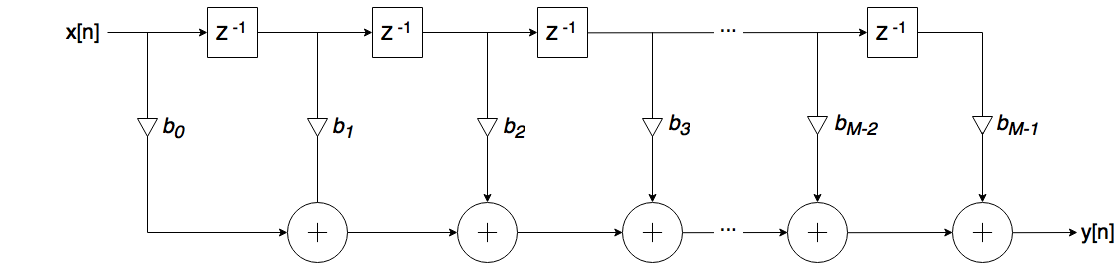
\includegraphics[width=\textwidth]{../figs/FIRFilter.png}
\caption{\label{fig:firfilter}Direct form representation of a N-order FIR-filter.}
\end{figure}
Even though the process of designing a \gls{fir}-filter might not be a trivial task, the implementation of an already designed filter is simple. As seen from \cref{eq:firfilterconv}, the filter can be described by the convolution formula, which implies that the filter can be implemented as convolution of the input function \textit{x(n)} with the impulse response function \textit{h(n)}.